\documentclass[a4paper,12pt]{report}
\usepackage{graphicx}
\usepackage{fancyhdr}
\usepackage{xcolor}

\pagestyle{fancy}

\fancyhf{} 
\fancyfoot[L]{\textcolor{teal}{\rule[0mm]{0.45\linewidth}{2pt}}} 
\fancyfoot[R]{\textcolor{teal}{\rule[0mm]{0.45\linewidth}{2pt}}} 

\fancyfoot[C]{\thepage}

\begin{document}

\begin{titlepage}
    \begin{center}
        \vspace*{2cm}

        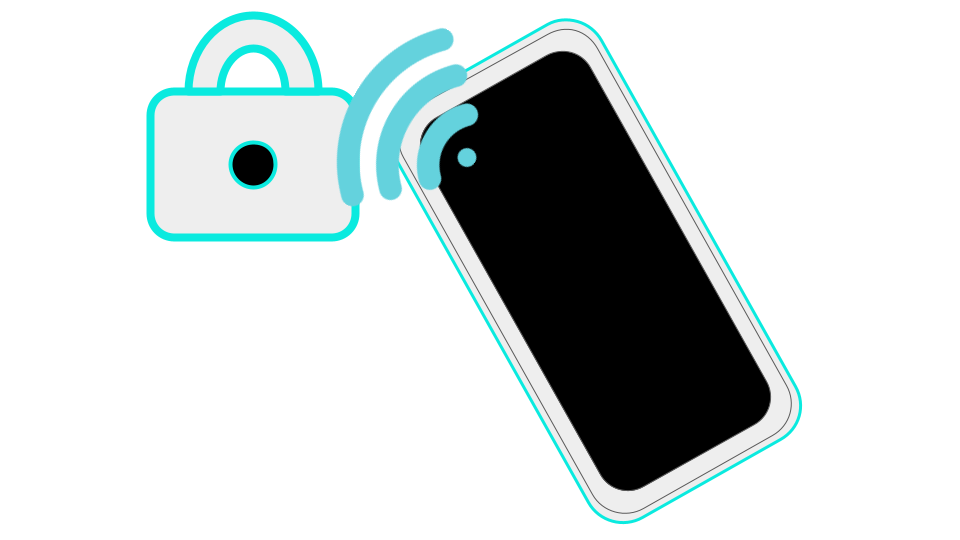
\includegraphics[width=0.8\textwidth]{slimg.png}\\[1cm]

        {\Huge \textbf{Smart Lock}}\\[0.5cm]
        {\textcolor{teal}{\Large A Cloud-Based Key}}\\[1.5cm]

        {\LARGE \textbf{Group 5}}\\[0.5cm]
        {\Large \textit{Names}}\\[2cm]

        {\Large \today}
    \end{center}
\end{titlepage}

\newpage
\pagenumbering{arabic}
\pagestyle{fancy}      

\section{Front Matter}
\subsection{Executive Summary}
Executive Summary Goes Here


\subsection{Ethics Statement for Smart Lock Project}
Our Smart Lock is designed to enhance security and convenience for users while upholding ethical standards in privacy, safety, and accessibility. We recognize our responsibility to develop and deploy technology that prioritizes ethical considerations in the following ways:

\textcolor{teal}{\subsubsection{Privacy and Data Protection}}
We are committed to safeguarding user privacy by:
\begin{itemize}
    \item Minimizing data collection to only essential information required for functionality.
    \item Implementing encryption and secure authentication methods to prevent unauthorized access.
    \item Ensuring that user data is never shared or sold to third parties without explicit consent.
\end{itemize}

\textcolor{teal}{\subsubsection{Security and Reliability}}
To maintain the integrity of the smart lock system, we will:
\begin{itemize}
    \item Use cybersecurity measures to prevent hacking and tampering.
    \item Regularly update software and firmware to address potential vulnerabilities.
    \item Ensure the lock functions reliably under various conditions to prevent accidental lockouts or failures.
\end{itemize}

\textcolor{teal}{\subsubsection{User Safety and Accessibility}}
We aim to create a system that is safe and inclusive by:
\begin{itemize}
    \item Designing intuitive user interfaces for easy access by individuals with different levels of technical proficiency.
    \item Ensuring compliance with accessibility standards for individuals with disabilities.
\end{itemize}

\textcolor{teal}{\subsubsection{Ethical Use and Non-Discrimination}}
The smart lock must be used ethically and responsibly by:
\begin{itemize}
    \item Preventing misuse that could lead to unauthorized surveillance or discrimination.
    \item Avoiding biases in authentication methods that may disadvantage certain user demographics.
\end{itemize}

\textcolor{teal}{\subsubsection{Transparency and Accountability}}
To uphold ethical standards, we will:
\begin{itemize}
    \item Clearly communicate to users how their data is handled and stored.
    \item Provide documentation on security features, risks, and best practices.
    \item Accept feedback and take responsibility for any ethical concerns that may arise during development and deployment.
\end{itemize}

By adhering to these ethical principles, we ensure that our Smart Lock product aligns with values of privacy, security, fairness, and social responsibility.

\subsection{Table of Contents}

\end{document}
